\documentclass{article}
\usepackage[utf8]{inputenc}
\usepackage[T1]{fontenc}
\usepackage{lmodern}
\usepackage{amsmath,amssymb,graphicx,booktabs,hyperref}
\usepackage{ComplexSystems}
\providecommand{\keywordsname}{Keywords}
\makeatletter\@ifundefined{keywords}{\newenvironment{keywords}{\par\vskip6pt\noindent{\small\itshape Keywords: }\small}{\par\vskip12pt}}{}\makeatother
\newcommand{\ncoreSingle}{22}
\newcommand{\ncoreRules}{57}
\newcommand{\ncorePairs}{243}
\newcommand{\nautSub}{36}
\newcommand{\nautSubN}{46}
\newcommand{\nautLight}{48}
\newcommand{\nautLightN}{194}
\newcommand{\nautRules}{13}
\newcommand{\nsilentSub}{21}
\newcommand{\nactiveSub}{37}
\newcommand{\nctwoRules}{25}
\newcommand{\nctwoN}{200}
\newcommand{\nctwoElastic}{101}
\newcommand{\nctwoTrans}{20}
\newcommand{\nctwoSup}{26}
\newcommand{\nctwoBubble}{25}
\newcommand{\nctwoUnres}{28}
\newcommand{\nstwoClean}{13}
\newcommand{\nstwoShadow}{12}
\newcommand{\nsthreePairs}{91}
\newcommand{\nsthreeClean}{45}
\newcommand{\nsthreeShadow}{45}
\newcommand{\nsthreeShadowRules}{14}
\newcommand{\nsthreeFoot}{45}
\newcommand{\nsthreeStatePos}{27}
\newcommand{\nsthreeStateOne}{19}
\newcommand{\nsthreeStateMed}{0.60}
\newcommand{\nonlyMin}{1.00}
\newcommand{\nonlyMax}{4.63}
\newcommand{\nsurvMed}{32}

\begin{document}
\title{The Shadow Knows: Interaction Records That\\ Outlive Their Carriers in Reversible\\ Second-Order Cellular Automata}
\author{\authname{Douglas Clark}\\[2pt]
\authadd{Independent Researcher}\\
\authadd{CITY, STATE ZIP, USA}\\
\authadd{clarkdd@gmail.com}
}
\markboth{Complex Systems}{Interaction Records That Outlive Their Carriers}
\maketitle
\begin{abstract}
In a reversible dynamics no information is destroyed, so the record of an interaction must persist somewhere. Where it goes is determined exactly in the 256 second-order extensions of the elementary cellular automata. Bounded, autonomous, slower-than-light coherences are first identified by frozen, outcome-blind searches and then collided. For each collision an exact ledger separates the information carried away by the outgoing coherences from the information left in the background. Every resolved coherence is then erased and a fresh probe is sent through the residue. Across \nsthreePairs{} collision pairs in 25 rules, pairs whose background returns to vacuum give the probe no information, while in all \nsthreeShadow{} pairs that leave a residue the probe recovers all of the information held only by the background, and in \nsthreeStatePos{} of them the probe coherence carries part of it away. All such shadows occur in rules with an oscillating vacuum.
\end{abstract}
\begin{keywords}
reversible cellular automata; second-order cellular automata; information dynamics; gliders; information storage; causal intervention
\end{keywords}
\section{Introduction}
Gliders in cellular automata are the standard example of coherent structures that carry and
process information: they transmit signals, and their collisions compute
\cite{park1986,boccara1991,hanson1997,adamatzky2012}. Local information dynamics has made this
quantitative. Gliders dominate information transfer, collisions dominate information modification,
and blinkers and background domains dominate information storage
\cite{lizier2008,lizier2010mod,lizier2012}. These results are statistical: they average over
ensembles of trajectories, and statistical transfer is not the same as causal influence
\cite{lizier2010caus,james2016}.

Here we ask an interventional version of the storage question in a setting where it has an exact
answer. In a \emph{reversible} automaton the global map is a bijection, so the information
distinguishing two interacting coherences before they meet cannot be lost. After the interaction
it must be carried by the outgoing coherences or by the background. If we erase the outgoing
coherences entirely, is a record of the interaction still present, and can a later coherence read
it? We call such a residual record a \emph{shadow}.

The question is motivated by the Information-Constraint Principle (ICP) \cite{clark2026icp}, which
treats physically effective information as interaction-formed constraint on reachable futures that
can persist beyond its original carrier. The present paper does not depend on that framework. It
reports frozen computational experiments on a complete, well-known rule family, including the rule
37R singled out by Wolfram for its localized structures \cite{wolfram2002}.

Our contributions are:
\begin{enumerate}
\item an outcome-blind identification of bounded, autonomous, slower-than-light coherences across
all 256 second-order rules;
\item an exact information ledger for collisions, separating what the outgoing coherences carry
from what the background holds;
\item a carrier-erasure intervention showing that the background's share is always present and
always fully recoverable by a passing probe, with an exact null in every rule whose background
returns to vacuum;
\item evidence that the probe coherence itself often carries the recovered record away.
\end{enumerate}

\section{Substrate and protocol}
\paragraph{Rules.} Cells $x_t(i)\in\{0,1\}$ on a ring evolve by
$x_{t+1}(i)=f\big(x_t(i-1),x_t(i),x_t(i+1)\big)\oplus x_{t-1}(i)$, where $f$ is any of the 256
elementary truth tables (Wolfram code). Every such rule is exactly invertible,
$x_{t-1}=f(x_t)\oplus x_{t+1}$ \cite{toffoli1990,wolfram2002}. The \emph{vacuum} is the orbit of the
all-zero state. It is silent when $f(000)=0$ and a homogeneous oscillation when $f(000)=1$. All
observables are differences from the matched vacuum evolved under the same rule.

\paragraph{Objects.} A coherence is a cluster of difference sites, on the union of both time layers
and with internal gaps of fewer than three sites, of width at most 8, that is exactly periodic up to
translation (pattern and vacuum phase both recur). Its velocity is the exact ratio of shift to period.
Its species is the set of states on its orbit.

\paragraph{Discipline.} Each test was written as a contract with fixed hypotheses and decision rules.
It was committed and tagged in git before the candidate family was evaluated, and the result was then
committed as a separate child commit. Exposure to earlier outcomes is disclosed in each contract.
Post-hoc analyses are labelled as such. Two runs crashed during serialization before any output; each
was refrozen with a disclosed one-line fix. One design was invalidated by its own control and replaced
(Section~\ref{sec:limits}).

\section{Coherences and their interactions}
\paragraph{Formation and autonomy.} A detector requiring an isolated core of width at most 8 that
persists for 64 ticks (confirmed on a larger ring) found \ncoreSingle{} rules in which a single
event produces such a core, and \ncoreRules{} rules (\ncorePairs{} rule--seed pairs) with seeds of
up to four bits. Most of these move at the causal limit. To separate genuine objects from features
of larger structures we cut each mature core out, including both time layers, and re-ran it alone in
the matched vacuum. \nautSub{} of \nautSubN{} slower-than-light cores (\nautRules{} rules) survived
unchanged, compared with \nautLight{} of \nautLightN{} light-speed cores (Fig.~\ref{fig:objects}). Typical
speeds are $1/2$ and $1/3$. A frozen hypothesis that slow objects require an active vacuum was
\emph{falsified} by an exhaustive two-layer seed search: \nsilentSub{} silent-vacuum rules host
slow bounded objects, compared with \nactiveSub{} active-vacuum rules.

\begin{figure}[t]\centering
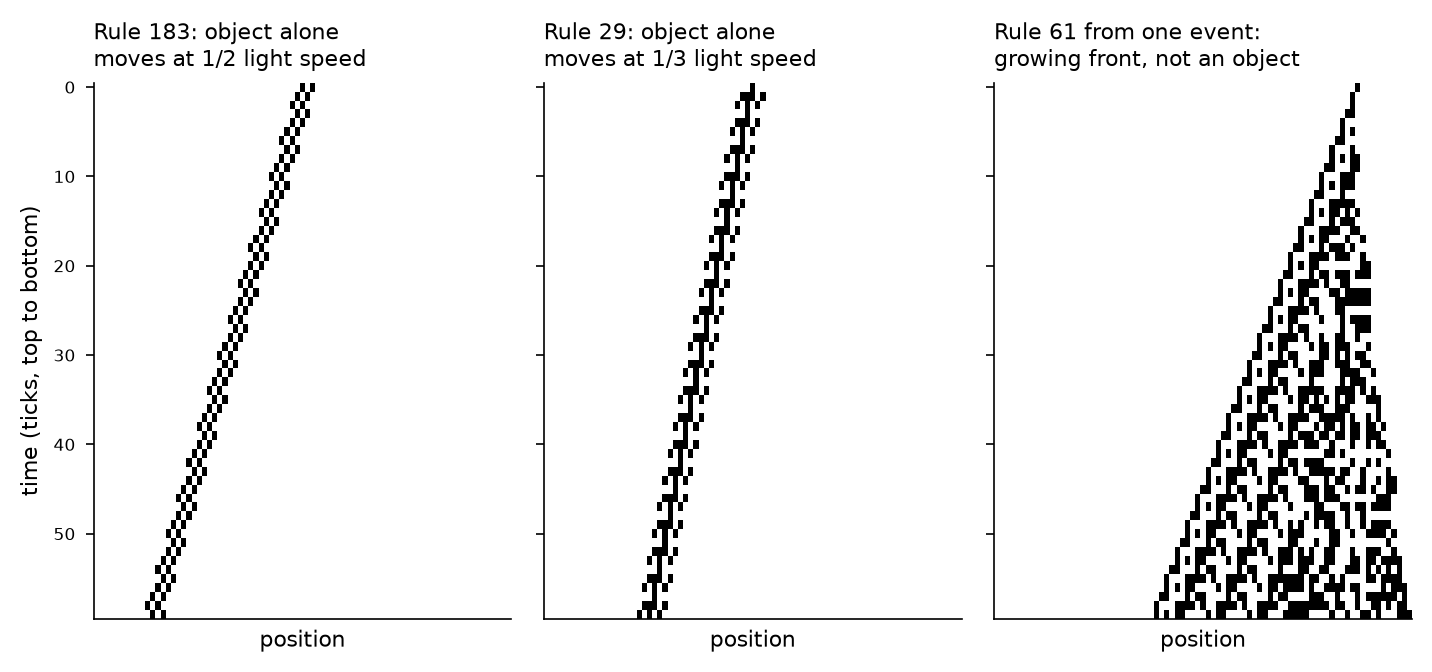
\includegraphics[width=\linewidth]{figures/fig1_objects.png}
\caption{Autonomous coherences cut out of their surroundings and run alone. Left and centre:
slower-than-light objects in rules 183 and 29. Right: a single event in rule 61 produces a growing
front, not an object. Time runs downward.}\label{fig:objects}
\end{figure}

\paragraph{Collisions.} Head-on collisions of the lowest-seed right- and left-moving objects
(\nctwoN{} collisions in \nctwoRules{} rules, eight impact phases each, all verified to make
contact) gave \nctwoElastic{} elastic outcomes, \nctwoTrans{} in which two different species
leave at the incoming speeds, \nctwoSup{} exact superpositions, \nctwoBubble{} in which the
collision opens an expanding domain of the opposite vacuum phase, and \nctwoUnres{} unresolved
outcomes. None annihilated, as reversibility requires (Fig.~\ref{fig:collisions}). In this design
every pair had opposite speeds of equal magnitude, so momentum-like conservation could not be tested.
Bubbles occurred only in active-vacuum rules, as predicted before the run.

\begin{figure}[t]\centering
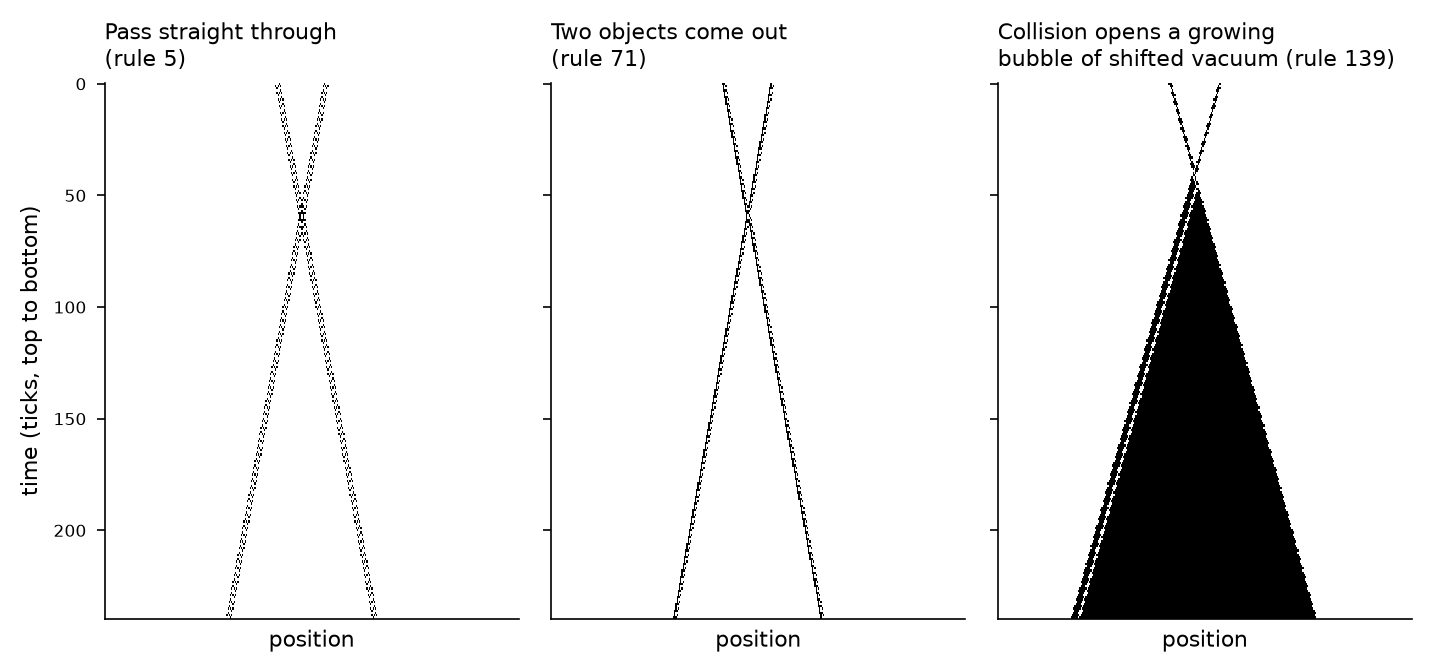
\includegraphics[width=\linewidth]{figures/fig2_collisions.png}
\caption{Three collision outcomes: exact pass-through, two coherences out, and a collision that
opens a growing domain of the opposite vacuum phase (black).}\label{fig:collisions}
\end{figure}

\section{The shadow}
\paragraph{Ledger.} For a fixed rule and pair, the 64 impact offsets form a uniform input set
($H(I)=6$ bits), and the dynamics is deterministic, so all entropies below are exact for that
ensemble. Let $O$ be the description (species, internal state, position) of all outgoing coherences at
$t=600$. Since the full state determines the input, $H(I\mid O)$ is exactly the information the
background holds and the coherences do not: the \emph{shadow-only} information.

\paragraph{Intervention.} At $t=600$ every resolved coherence is erased (both layers set to vacuum),
leaving only the residue. A probe, an exact copy of the right-moving object's free-flight state, is
written at one fixed site outside every shadow for all 64 offsets, so its starting position carries no
information about the input. The worlds with and without the probe are run for 1500 further ticks.
The \emph{footprint} $Y$ is their difference. The \emph{probe state} $Y_p$ is the set of resolved
coherences in the region where they differ. We report $I(I;Y\mid O)/H(I\mid O)$ and
$I(I;Y_p\mid O)/H(I\mid O)$.

\paragraph{Results.} The null holds exactly: in all \nsthreeClean{} pairs whose background
returns to vacuum after erasure, both readouts are zero. In all \nsthreeShadow{} pairs that leave a
residue (\nsthreeShadowRules{} rules) the footprint ratio is exactly 1. The probe's passage
determines every bit of the shadow-only information, which ranges from \nonlyMin{} to
\nonlyMax{} bits (Fig.~\ref{fig:ledger}, left). The record is also often carried out by a coherence:
the probe-state ratio is positive in \nsthreeStatePos{} of \nsthreeShadow{} pairs and equal to 1 in
\nsthreeStateOne{}, with median \nsthreeStateMed{} (Fig.~\ref{fig:ledger}, right). A coherence of the
probe's own species leaves in a median of \nsurvMed{} of 64 runs. All shadow rules have an active
vacuum. An earlier one-pair-per-rule version of the test (\nstwoShadow{} shadow rules, \nstwoClean{}
clean) gave the same footprint result.

\begin{figure}[t]\centering
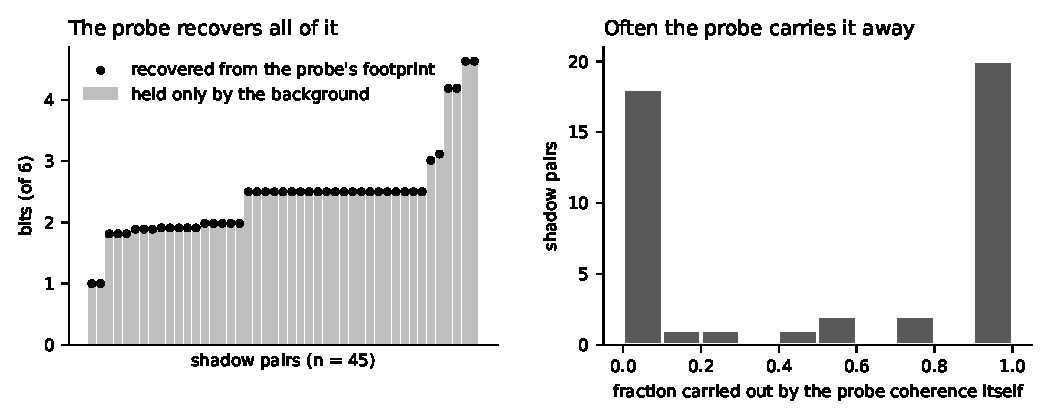
\includegraphics[width=\linewidth]{figures/fig3_ledger.pdf}
\caption{Left: information held only by the background after a collision (bars) and the amount
recovered from a probe's footprint after the carriers were erased (dots), for every shadow pair.
Right: fraction of that information carried out by the probe coherence itself.}\label{fig:ledger}
\end{figure}

\section{Related work}
Reversible, information-conserving automata and the second-order construction are classical
\cite{fredkin1982,toffoli1987,toffoli1990}. Rule 37R and its structures were described by Wolfram
\cite{wolfram2002}, and exactly solvable reversible automata with interacting quasiparticles,
notably the reversible Rule 54, are now well understood
\cite{buca2021,klobas2022,prosen2023,wilkinson2022}. That work analyses scattering and
thermalization, not records left behind once the carriers are gone. Particles as information carriers
and domain walls are formalized in computational mechanics
\cite{hanson1992,hanson1997,hordijk2001,pivato2007,rupe2018}. The closest precedent is local
information dynamics, which identifies background domains as the dominant information storage in
irreversible elementary automata \cite{lizier2012}. Our contribution is interventional and exact
rather than statistical, in line with causal information-flow measures \cite{ay2008,lizier2010caus}.
Collision-based computing uses designed collisions that write stationary memory read by later
gliders \cite{adamatzky2012,martinez2006,martinez2011,martinez2012}. The shadows here are
emergent vacuum-phase residues, not designed localizations. Information left in an environment and
read later has also been studied as stigmergy \cite{klyubin2004} and as outsourced memory through
niche construction \cite{lee2022}.

\section{Limitations and failed runs}\label{sec:limits}
The ensembles are finite (64 offsets per pair, at most four pairs per rule) and one-dimensional.
The entropies are exact for these ensembles, not capacities over all collisions. The footprint is a
whole-world readout. The probe-state readout is stricter but depends on our object definition (width
at most 8, exact periodicity). Every shadow observed so far occurs in an active-vacuum rule, so whether
silent vacua can hold shadows remains open.

The path included failures that shaped the final design. An inherited proto-object detector
was passed formally by 16 rules that formed only expanding wedges. A collision classifier first
counted non-meeting pairs as pass-throughs and mislabelled radiation; a bubble-wall speed
measurement was invalid. An object extractor that clustered on one time layer created a spurious
null; it was fixed by clustering on both layers. A first shadow design erased carriers before they had
separated and failed its own control. The ``active vacuum is required for slow objects'' hypothesis
was falsified. All are recorded in the repository with their commits.

\section{Discussion}
Reversibility forces the question ``where did the information go?'' to have an exact answer, and
the answer has two parts. Outgoing coherences carry the record mainly relationally, through where
they are. When the background is itself dynamic, part of the record is deposited there. That deposit
is not inert. With the original carriers erased it fully determines how a later coherence's passage
reshapes the future, and often the later coherence leaves carrying it. In the vocabulary that
motivated this study, the residue is interaction-formed constraint on reachable futures that has
outlived its carriers \cite{clark2026icp}. Open questions include whether silent vacua can hold
shadows, how shadow capacity scales with collision diversity, and whether the result extends to
two-dimensional and quantum reversible dynamics.

\section*{Data and Code Availability}
All code, frozen contracts, seals and results are in the Iota repository (\url{https://github.com/fmertz55/iota}) under
\path{src/minimal_realization_reversible}, \path{docs/ICP_MIR_REVERSIBLE_*}, and
\path{output/minimal_realization/MIR-REVERSIBLE-*}. Each contract is tagged
\texttt{mir-reversible-*-frozen}. Numbers in this paper are generated from the committed result files
by \path{scripts/build_shadow_paper_assets.py}.

\section*{Acknowledgments}
The author used OpenAI Codex and Anthropic Claude for AI-assisted literature triage, drafting, code review and LaTeX editing. The author reviewed and verified the sources, calculations, code, claims and final text, and takes full responsibility for the content. No funding was received for this work.
\begin{thebibliography}{99}
\bibitem{park1986}
J. K. Park, K. Steiglitz and W. P. Thurston, ``Soliton-like behavior in automata,'' \textit{Physica D: Nonlinear Phenomena}, \textbf{19}(3), 1986 pp. 423--432. doi:10.1016/0167-2789(86)90068-0.

\bibitem{boccara1991}
N. Boccara, J. Nasser and M. Roger, ``Particlelike structures and their interactions in spatiotemporal patterns generated by one-dimensional deterministic cellular-automaton rules,'' \textit{Physical Review A}, \textbf{44}(2), 1991 pp. 866--875. doi:10.1103/physreva.44.866.

\bibitem{hanson1997}
J. E. Hanson and J. P. Crutchfield, ``Computational mechanics of cellular automata: An example,'' \textit{Physica D: Nonlinear Phenomena}, \textbf{103}(1-4), 1997 pp. 169--189. doi:10.1016/s0167-2789(96)00259-x.

\bibitem{adamatzky2012}
A. Adamatzky and J. Durand-Lose, ``Collision-Based Computing,'' in \textit{Handbook of Natural Computing}, Springer Berlin Heidelberg, 2012 pp. 1949--1978. doi:10.1007/978-3-540-92910-9\_58.

\bibitem{lizier2008}
J. T. Lizier, M. Prokopenko and A. Y. Zomaya, ``Local information transfer as a spatiotemporal filter for complex systems,'' \textit{Physical Review E}, \textbf{77}(2), 2008. doi:10.1103/physreve.77.026110.

\bibitem{lizier2010mod}
J. T. Lizier, M. Prokopenko and A. Y. Zomaya, ``Information modification and particle collisions in distributed computation,'' \textit{Chaos: An Interdisciplinary Journal of Nonlinear Science}, \textbf{20}(3), 2010. doi:10.1063/1.3486801.

\bibitem{lizier2012}
J. T. Lizier, M. Prokopenko and A. Y. Zomaya, ``Local measures of information storage in complex distributed computation,'' \textit{Information Sciences}, \textbf{208}, 2012 pp. 39--54. doi:10.1016/j.ins.2012.04.016.

\bibitem{lizier2010caus}
J. T. Lizier and M. Prokopenko, ``Differentiating information transfer and causal effect,'' \textit{The European Physical Journal B}, \textbf{73}(4), 2010 pp. 605--615. doi:10.1140/epjb/e2010-00034-5.

\bibitem{james2016}
R. G. James, N. Barnett and J. P. Crutchfield, ``Information Flows? A Critique of Transfer Entropies,'' \textit{Physical Review Letters}, \textbf{116}(23), 2016. doi:10.1103/physrevlett.116.238701.

\bibitem{clark2026icp}
D. Clark, ``The Constrained Future: A Testable Information-Constraint Principle for Persistent Organization,'' submitted to \textit{BioSystems}, 2026.

\bibitem{wolfram2002}
S. Wolfram, \textit{A New Kind of Science}, Champaign, IL: Wolfram Media, 2002.

\bibitem{toffoli1990}
T. Toffoli and N. H. Margolus, ``Invertible cellular automata: A review,'' \textit{Physica D: Nonlinear Phenomena}, \textbf{45}(1-3), 1990 pp. 229--253. doi:10.1016/0167-2789(90)90185-r.

\bibitem{fredkin1982}
E. Fredkin and T. Toffoli, ``Conservative logic,'' \textit{International Journal of Theoretical Physics}, \textbf{21}(3-4), 1982 pp. 219--253. doi:10.1007/bf01857727.

\bibitem{toffoli1987}
T. Toffoli and N. Margolus, \textit{Cellular Automata Machines: A New Environment for Modeling}, The MIT Press, 1987. doi:10.7551/mitpress/1763.001.0001.

\bibitem{buca2021}
B. Buča, K. Klobas and T. Prosen, ``Rule 54: exactly solvable model of nonequilibrium statistical mechanics,'' \textit{Journal of Statistical Mechanics: Theory and Experiment}, \textbf{2021}(7), 2021 pp. 074001. doi:10.1088/1742-5468/ac096b.

\bibitem{klobas2022}
K. Klobas and T. Prosen, ``On two reversible cellular automata with two particle species,'' \textit{Journal of Physics A: Mathematical and Theoretical}, \textbf{55}(9), 2022 pp. 094003. doi:10.1088/1751-8121/ac3ebc.

\bibitem{prosen2023}
T. Prosen, ``On Two Non-Ergodic Reversible Cellular Automata, One Classical, the Other Quantum,'' \textit{Entropy}, \textbf{25}(5), 2023 pp. 739. doi:10.3390/e25050739.

\bibitem{wilkinson2022}
J. W. P. Wilkinson, T. Prosen and J. P. Garrahan, ``Exact solution of the `Rule 150' reversible cellular automaton,'' \textit{Physical Review E}, \textbf{105}(3), 2022. doi:10.1103/physreve.105.034124.

\bibitem{hanson1992}
J. E. Hanson and J. P. Crutchfield, ``The attractor--basin portrait of a cellular automaton,'' \textit{Journal of Statistical Physics}, \textbf{66}(5-6), 1992 pp. 1415--1462. doi:10.1007/bf01054429.

\bibitem{hordijk2001}
W. Hordijk, C. R. Shalizi and J. P. Crutchfield, ``Upper bound on the products of particle interactions in cellular automata,'' \textit{Physica D: Nonlinear Phenomena}, \textbf{154}(3-4), 2001 pp. 240--258. doi:10.1016/s0167-2789(01)00252-4.

\bibitem{pivato2007}
M. Pivato, ``Defect particle kinematics in one-dimensional cellular automata,'' \textit{Theoretical Computer Science}, \textbf{377}(1-3), 2007 pp. 205--228. doi:10.1016/j.tcs.2007.03.014.

\bibitem{rupe2018}
A. Rupe and J. P. Crutchfield, ``Local causal states and discrete coherent structures,'' \textit{Chaos: An Interdisciplinary Journal of Nonlinear Science}, \textbf{28}(7), 2018. doi:10.1063/1.5021130.

\bibitem{ay2008}
N. Ay and D. Polani, ``Information Flows in Causal Networks,'' \textit{Advances in Complex Systems}, \textbf{11}(1), 2008 pp. 17--41. doi:10.1142/s0219525908001465.

\bibitem{martinez2006}
G. J. Martínez, A. Adamatzky and H. V. McIntosh, ``Phenomenology of glider collisions in cellular automaton Rule 54 and associated logical gates,'' \textit{Chaos, Solitons \& Fractals}, \textbf{28}(1), 2006 pp. 100--111. doi:10.1016/j.chaos.2005.05.013.

\bibitem{martinez2011}
G. J. Mart\'{\i}nez, A. Adamatzky, C. R. Stephens and A. F. Hoeflich, ``Cellular Automaton Supercolliders,'' \textit{International Journal of Modern Physics C}, \textbf{22}(4), 2011 pp. 419--439. doi:10.1142/s0129183111016348.

\bibitem{martinez2012}
G. J. Mart\'{\i}nez, A. Adamatzky, F. Chen and L. Chua, ``On Soliton Collisions between Localizations in Complex Elementary Cellular Automata: Rules 54 and 110 and Beyond,'' \textit{Complex Systems}, \textbf{21}(2), 2012 pp. 117--142. doi:10.25088/complexsystems.21.2.117.

\bibitem{klyubin2004}
A. S. Klyubin, D. Polani and C. L. Nehaniv, ``Tracking Information Flow through the Environment: Simple Cases of Stigmergy,'' in \textit{Artificial Life IX}, The MIT Press, 2004 pp. 563--568. doi:10.7551/mitpress/1429.003.0095.

\bibitem{lee2022}
E. D. Lee, J. C. Flack and D. C. Krakauer, ``Outsourcing Memory Through Niche Construction,'' bioRxiv preprint, 2022. doi:10.1101/2022.09.01.506204.
\end{thebibliography}
\end{document}
